% =====================================================================
% Deep Double Descent - COMP34312 Poster Coursework
% A2 portrait, beamerposter, customised UoM purple theme.
% Compile: pdflatex poster.tex
% =====================================================================
\documentclass[final]{beamer}

\usepackage[orientation=portrait,size=a2,scale=1.00]{beamerposter}
\usepackage{lmodern}
\usepackage[T1]{fontenc}
\usepackage[utf8]{inputenc}
\usepackage{amsmath,amssymb,amsthm,bm,mathtools}
\usepackage{xcolor}
\usepackage{graphicx}
\usepackage{tikz}
\usepackage{microtype}
\usepackage{booktabs}
\usepackage[english]{babel}
\usepackage{calc}
\usepackage{ragged2e}
\usetikzlibrary{shapes,arrows.meta,positioning,calc,backgrounds,fit,decorations.pathreplacing}

% ----- Colours: University of Manchester palette + supporting accents -----
\definecolor{uompurple}{HTML}{660099}     % Primary UoM purple
\definecolor{uompurpleDark}{HTML}{3F0066} % Deep variant for headers
\definecolor{uompurplePale}{HTML}{F2EAF7} % Background tint
\definecolor{uomgrey}{HTML}{2A2A33}       % Body text
\definecolor{uommuted}{HTML}{555A66}      % Captions/secondary
\definecolor{uomline}{HTML}{D9DCE5}       % Dividers
\definecolor{accentcoral}{HTML}{D1495B}   % Critical regime / warnings
\definecolor{accentteal}{HTML}{087E8B}    % Underparameterized
\definecolor{accentgreen}{HTML}{2E7D32}   % Overparameterized / good
\definecolor{accentgold}{HTML}{B98300}    % Caveats / boundary
\definecolor{accentblue}{HTML}{2D6CDF}    % Sample-wise

% ----- Theme overrides -----
\setbeamercolor{normal text}{fg=uomgrey,bg=white}
\setbeamercolor{block title}{fg=white,bg=uompurple}
\setbeamercolor{block body}{fg=uomgrey,bg=white}
\setbeamerfont{block title}{size=\Large,series=\bfseries}
\setbeamerfont{block body}{size=\normalsize}
\setbeamertemplate{itemize items}[circle]
\setbeamertemplate{itemize item}{\textcolor{uompurple}{\textbullet}}
\setbeamertemplate{itemize subitem}{\textcolor{uommuted}{\(\cdot\)}}
\setbeamertemplate{navigation symbols}{}

% Rounded block titles + body, similar to UoM template but cleaner
\setbeamertemplate{block begin}{
  \par\vskip0.6ex
  \begin{beamercolorbox}[rounded=true,leftskip=0.6cm,colsep*=0.6ex,wd=\linewidth]{block title}%
    \usebeamerfont*{block title}\insertblocktitle%
  \end{beamercolorbox}%
  \nointerlineskip\vskip-0.3ex%
  \usebeamerfont{block body}%
  \begin{beamercolorbox}[rounded=true,leftskip=0.4cm,rightskip=0.4cm,colsep*=0.6ex,sep=0.5ex,vmode]{block body}%
    \vbox{}\vskip-0.3ex%
}
\setbeamertemplate{block end}{%
  \end{beamercolorbox}\vskip0.4ex%
}

% ----- Custom commands -----
% Highlight keyword
\newcommand{\kw}[1]{\textcolor{uompurple}{\textbf{#1}}}
% Eyebrow above block title
\newcommand{\eyebrow}[1]{{\color{uompurple}\footnotesize\bfseries\MakeUppercase{#1}}\par\vspace{-0.2ex}}
% Single-line callout / takeaway
\newcommand{\takeaway}[1]{%
  \begin{center}\colorbox{uompurplePale}{\parbox{0.96\linewidth}{\centering\itshape\textcolor{uompurpleDark}{\textbf{#1}}}}\end{center}}
% Prominent final takeaway: full-width purple band with white bold text
\newcommand{\bigtakeaway}[1]{%
  \par\noindent\colorbox{uompurple}{\parbox{\linewidth-2\fboxsep}{\centering\bfseries\normalsize\color{white}\,#1\,}}\par}
% Coloured chip
\newcommand{\chip}[2]{\textcolor{white}{\colorbox{#1}{\strut~\bfseries\small #2~}}}
% Math operators / shortcuts
\newcommand{\E}{\mathbb{E}}
\newcommand{\T}{\mathcal{T}}
\newcommand{\D}{\mathcal{D}}
\newcommand{\F}{\mathcal{F}}
\newcommand{\Sset}{\mathcal{S}}
\newcommand{\HypBox}[1]{%
  \par\noindent\colorbox{uompurplePale}{\parbox{\linewidth-2\fboxsep}{\small #1}}}

% ----- Title block content -----
\title{Deep Double Descent}
\subtitle{Where Bigger Models, Longer Training, and More Data Can Hurt}
\author{}
\institute{}

% Custom headline: logo on left, title block centred
\setbeamertemplate{headline}{
  \leavevmode
  \begin{beamercolorbox}[wd=\paperwidth]{headline}
    \vskip0.5cm
    \begin{minipage}[c]{0.13\paperwidth}
      \hspace*{0.4cm}
\includegraphics[height=5.4cm]{Manchester_Logo}
    \end{minipage}%
    \begin{minipage}[c]{0.74\paperwidth}
      \centering
      {\color{uomgrey}\fontsize{60}{66}\selectfont\bfseries Deep Double Descent}\\[0.2ex]
      {\color{uompurple}\fontsize{26}{32}\selectfont\bfseries Where bigger models, longer training, and more data can hurt}\\[0.4ex]
      {\color{uommuted}\fontsize{17}{22}\selectfont COMP34312 \textbar{} Mathematical Topics in Machine Learning \textbar{} Poster Coursework}\\[0.0ex]
      {\color{uommuted}\fontsize{17}{22}\selectfont \textbf{Group:} \textit{Ayush Kumar} \textbar{} \textit{Jacob Yip} \textbar{} \textit{Harshita Dassani}}
    \end{minipage}%
    \begin{minipage}[c]{0.13\paperwidth}\hspace*{0pt}\end{minipage}
    \vskip0.4cm
  \end{beamercolorbox}
  \begin{beamercolorbox}[wd=\paperwidth,ht=0.16cm]{}\color{uompurple}\rule{\paperwidth}{0.16cm}\end{beamercolorbox}
}

\setbeamertemplate{footline}{}

\begin{document}
\begin{frame}[t]{}
\vspace*{-0.5cm}

% =====================================================================
% O/P/A/C STRIP (full width, compact 30-second story)
% =====================================================================
\par\noindent\colorbox{uompurplePale}{\parbox{\linewidth-2\fboxsep}{%
\small
\begin{tabular}{@{}p{2.4cm}@{\hspace{0.4em}}p{\dimexpr\linewidth-3.0cm}@{}}
\textcolor{uompurple}{\textbf{Objective}} & Explain why test error can peak \emph{near interpolation} and then fall again.\\
\textcolor{uompurple}{\textbf{Problem}} & Classical bias\textendash variance theory predicts one U-shape; modern overparameterised nets interpolate yet generalise.\\
\textcolor{uompurple}{\textbf{Approach}} & Sweep width, training time, samples, noise, optimiser, regularisation; track test \emph{and} train error.\\
\textcolor{uompurple}{\textbf{Contribution}} & Nakkiran et al.\ unify model-wise, epoch-wise, and sample-wise double descent via \kw{Effective Model Complexity} (EMC).\\
\end{tabular}%
}}
\vspace{0.05cm}

% =====================================================================
% 1. HERO BLOCK: Beyond the U-Curve (full width)
% =====================================================================
\begin{block}{1.~From the textbook U-curve to the double-descent peak}
\begin{columns}[T,onlytextwidth]
\begin{column}{0.58\linewidth}
\centering
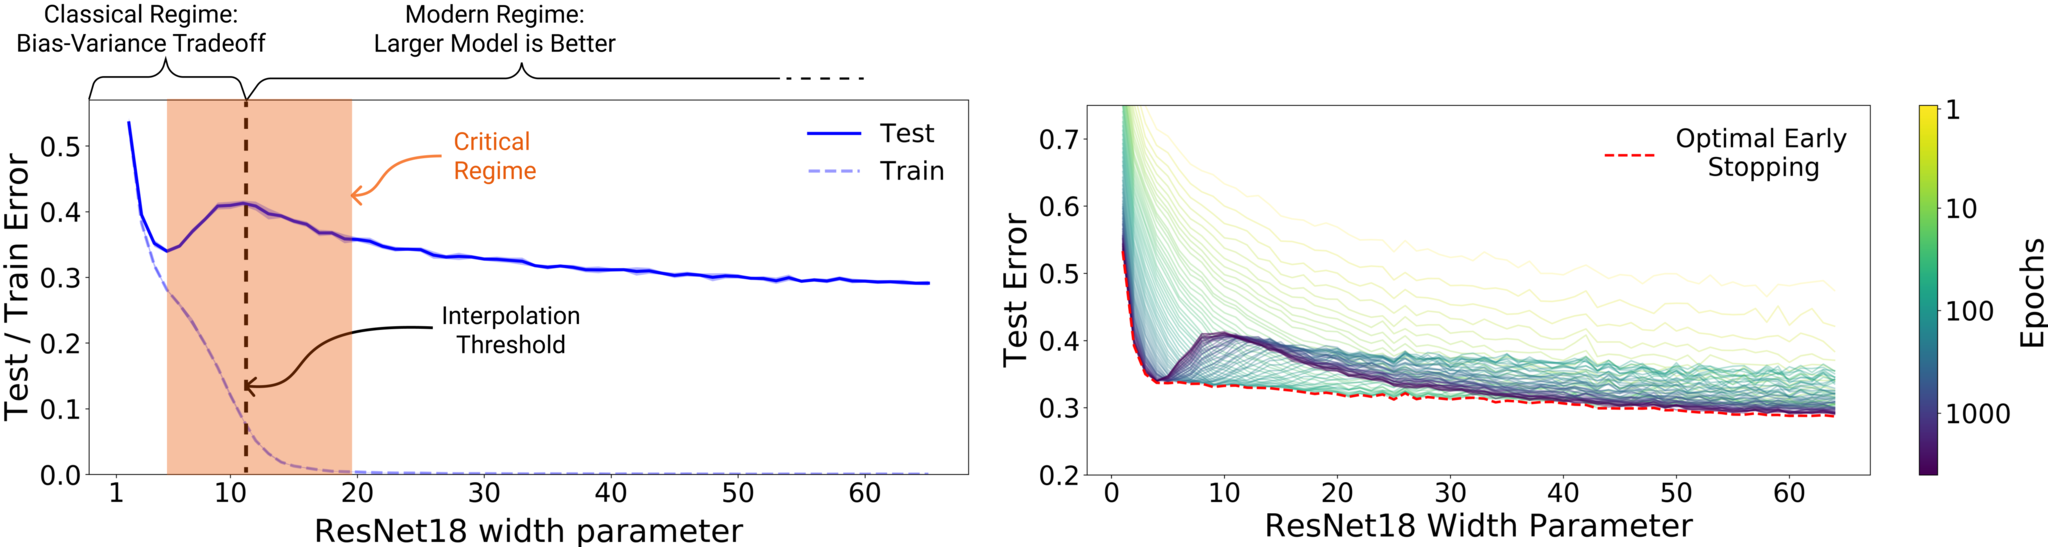
\includegraphics[width=0.98\linewidth,height=6.0cm,keepaspectratio]{assets/errorvscomplexity.png}\\[0.1ex]
{\scriptsize\color{uommuted}\textbf{Fig.~1, Nakkiran et al.\ (2019).} \textbf{Left:} test error on ResNet18s, varying width, CIFAR-10 + 15\% label noise. \textbf{Right:} test error coloured by training epoch; dashed red curve denotes optimal early stopping.}
\end{column}\hspace{0.02\linewidth}%
\begin{column}{0.38\linewidth}
\eyebrow{Thesis}
{\color{uomgrey}\textbf{For modern training procedures the population-risk curve exhibits \emph{two} descents,} separated by a sharp peak at the \kw{interpolation threshold} at which the procedure first fits the training set exactly.}\\[0.3ex]
\eyebrow{Beyond Section 5.3}
\small
The lecture introduces the phenomenon and links it to implicit regularisation. We extend this by substituting \emph{parameter count} with \kw{Effective Model Complexity} (EMC) -- the capacity of the entire training procedure \(\T\) -- and demonstrating that the second descent occurs \kw{model-wise}, \kw{epoch-wise}, and \kw{sample-wise}, unified under the \kw{Generalised Double Descent Hypothesis}.
\end{column}
\end{columns}
\end{block}

\vspace{-0.25cm}

% =====================================================================
% TWO-COLUMN ROW: Setting & Notation | Definition & Hypothesis
% =====================================================================
\begin{columns}[T,onlytextwidth]

% --------- LEFT COLUMN ---------
\begin{column}{0.485\linewidth}

\begin{block}{2.~Setting: the lecture decomposition we extend}
Following the course notation (Notes \S\,5.1, Eqs.~68 to 73):
\[\hat f \leftarrow \mathcal{A}(\F;\Sset),\qquad
  R(f) := \E_{\bm{xy}}[\ell(\bm{y},f(\bm{x}))],\qquad
  \widehat R(f,\Sset) := \tfrac{1}{n}\sum_{i=1}^{n}\ell(\bm{y}_i,f(\bm{x}_i)).\]
The excess risk decomposes into three statistically meaningful gaps:
\[\underbrace{R(\hat f) - R(y^{*})}_{\text{excess risk}}
  = \underbrace{R(\hat f) - R(f_{\mathrm{erm}})}_{\text{\color{accentteal}\textbf{optimisation}}}
  + \underbrace{R(f_{\mathrm{erm}}) - R(f^{*})}_{\text{\color{accentgold}\textbf{estimation}}}
  + \underbrace{R(f^{*}) - R(y^{*})}_{\text{\color{accentblue}\textbf{approximation}}}.\]
The classical bias-variance trade-off bundles \emph{approximation + part of estimation} into \kw{bias} and the rest into \kw{variance}; what the lecture summary calls \emph{incomplete}, not wrong.

\begin{itemize}\setlength\itemsep{0.2ex}
\item \kw{Lecture U-curve} (Notes Fig.~17) holds \(\F,\mathcal{A}\) fixed and grows \(\F\).
\item \kw{Paper's pivot:} treat the \emph{whole procedure} \(\T\!=\!(\F,\mathcal{A},\text{epochs},\text{reg.},\text{labels})\) as the single object whose capacity matters, so optimisation, estimation, and labels jointly determine the peak.
\end{itemize}
\end{block}

\end{column}

% --------- RIGHT COLUMN ---------
\begin{column}{0.485\linewidth}

\begin{block}{3.~Definition + Hypothesis (Nakkiran et al.\ 2019)}
\eyebrow{Definition 1: Effective Model Complexity}
A \kw{training procedure} \(\T\) maps any labelled train set \(S = \{(\bm{x}_i,\bm{y}_i)\}_{i=1}^{n}\) to a classifier \(\T(S)\). For an error tolerance \(\varepsilon>0\),
\[\boxed{\;\mathrm{EMC}_{\D,\varepsilon}(\T)\;:=\;\max\bigl\{\,n\;\bigm|\;\E_{S\sim\D^{n}}\bigl[\mathrm{Error}_{S}(\T(S))\bigr]\le\varepsilon\,\bigr\}\;}\]
i.e.\ the largest sample size on which \(\T\) can still drive train error below \(\varepsilon\). Note that \(\mathrm{EMC}\) depends on the optimiser, training time, augmentation and labels, not just on the architecture.

\vspace{0.4ex}
\eyebrow{Hypothesis 1: Generalised Double Descent}
For ``natural'' \(\D\), neural-network procedures \(\T\), and small \(\varepsilon\) (the paper uses \(\varepsilon=0.1\)):
\begin{itemize}\setlength\itemsep{0.3ex}
\item[\chip{accentteal}{$\mathrm{EMC}\!\ll\! n$}] \kw{Under-parameterised:} any change to \(\T\) that \emph{increases} EMC \emph{decreases} test error.
\item[\chip{accentcoral}{$\mathrm{EMC}\!\approx\! n$}] \kw{Critically parameterised:} the sign of the same change is \emph{indeterminate}.
\item[\chip{accentgreen}{$\mathrm{EMC}\!\gg\! n$}] \kw{Over-parameterised:} any change to \(\T\) that \emph{increases} EMC \emph{decreases} test error.
\end{itemize}

\HypBox{\textbf{Why this is a hypothesis, not a theorem.} \(\varepsilon\) and the words ``sufficiently smaller / larger'' are heuristic; the critical-interval width is not formally specified for deep nets. \kw{EMC is operational, not predictive}: there is no closed form, so the peak location must be \emph{measured}, not derived.}
\end{block}

\end{column}
\end{columns}

\vspace{-0.25cm}

% =====================================================================
% HERO BLOCK 2: Main heatmap evidence (full width)
% =====================================================================
\begin{block}{4.~Main empirical evidence: model-wise \(\times\) epoch-wise double descent}
\begin{columns}[T,onlytextwidth]
\begin{column}{0.34\linewidth}
\centering
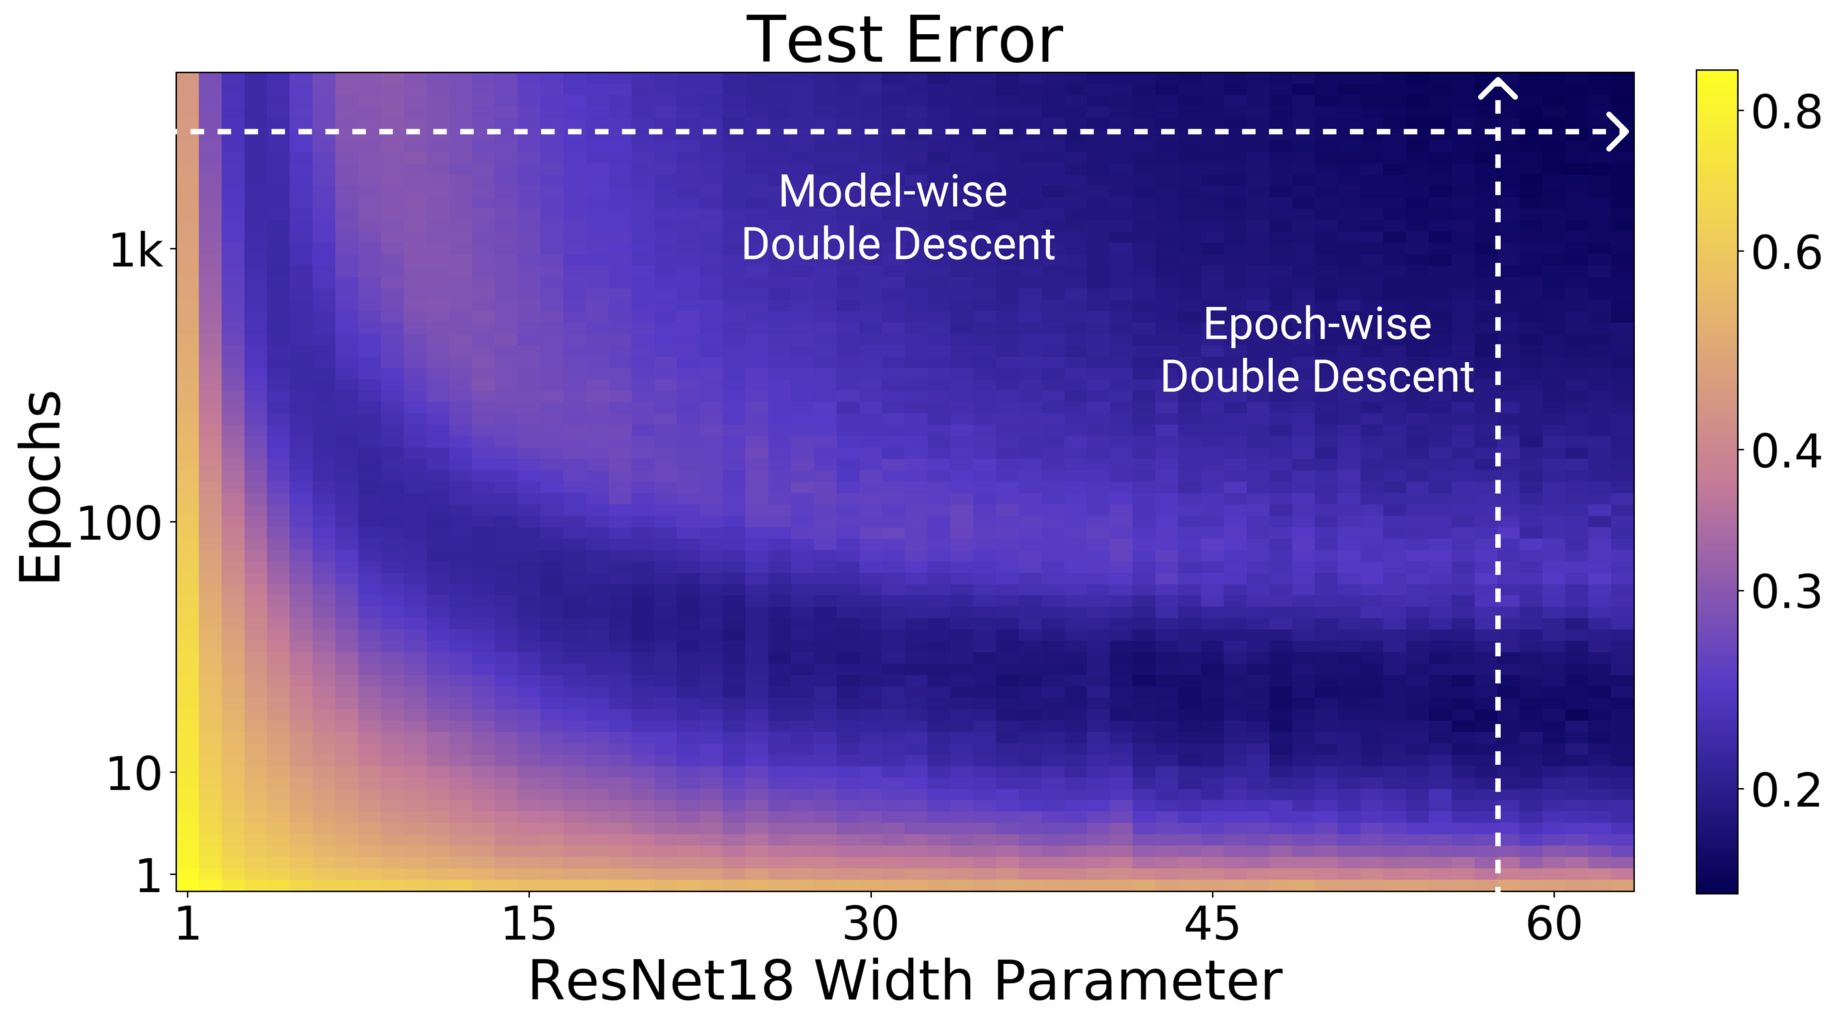
\includegraphics[width=0.98\linewidth,height=5.2cm,keepaspectratio]{assets/Intro-ocean-test.png}\\[0.1ex]
{\scriptsize\color{uommuted}\textbf{Fig.~2 (left), Nakkiran et al.\ \textemdash{} test error.} Test error attains \(\approx\) 0.47 at width \(k\!\approx\!10\) and decreases to \(\approx\) 0.24 at \(k\!=\!64\).}
\end{column}\hspace{0.01\linewidth}%
\begin{column}{0.34\linewidth}
\centering
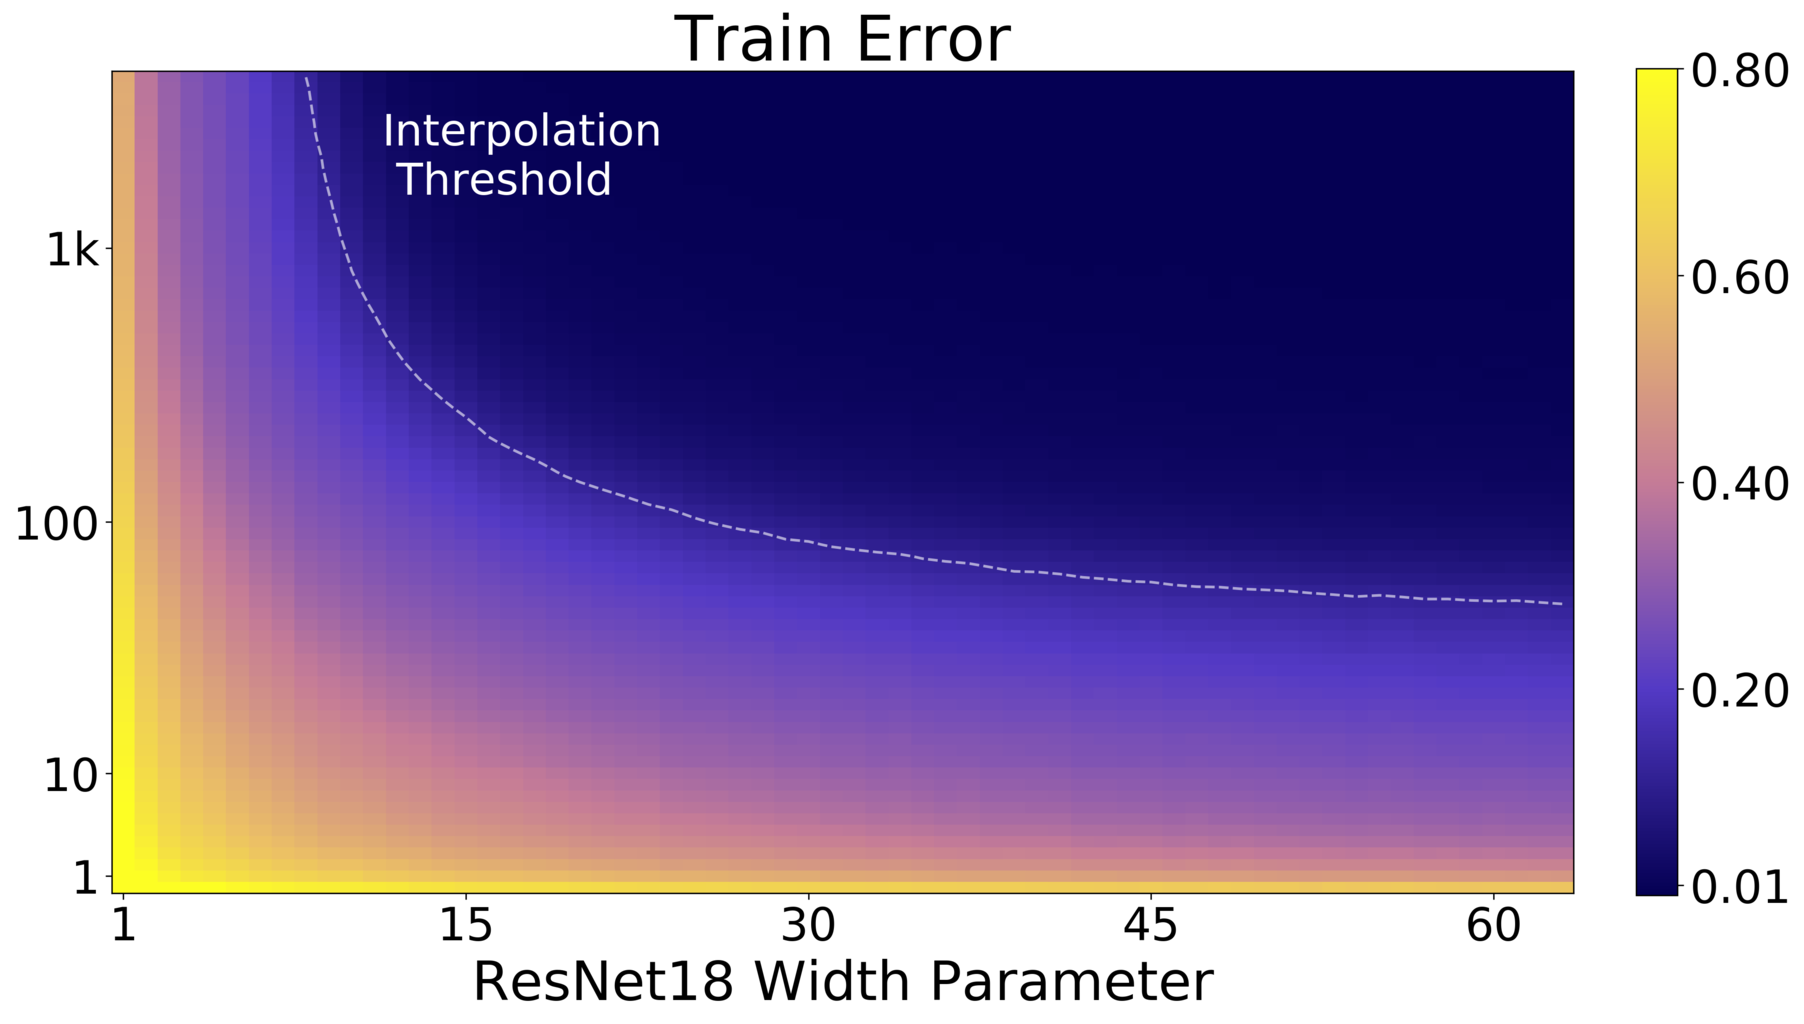
\includegraphics[width=0.98\linewidth,height=5.2cm,keepaspectratio]{assets/Rn-cifar10-p15-adam-aug-train.png}\\[0.1ex]
{\scriptsize\color{uommuted}\textbf{Fig.~2 (right), train error.} Dashed curve denotes the interpolation threshold (\(\widehat R\!\to\!0\)).}
\end{column}\hspace{0.01\linewidth}%
\begin{column}{0.30\linewidth}
\eyebrow{Reading the heatmaps}
\small
\begin{itemize}\setlength\itemsep{0.2ex}
\item \kw{Same axes:} ResNet18 width \(k\!\in\![1,64]\) vs training epochs (log).
\item \kw{Horizontal slice}: \chip{accentcoral}{model-wise} peak as width grows. \kw{Vertical slice}: \chip{accentteal}{epoch-wise} peak as training continues.
\item \kw{Key alignment:} the bright \emph{test} ridge sits on the \emph{train} interpolation curve, so the peak is \emph{at} the threshold.
\end{itemize}
\eyebrow{Setup + key numbers (paper \S\,4)}
\footnotesize
ResNet18, CIFAR-10, \kw{15\% label noise}, augmentation, Adam (lr 1e-4), 4k epochs. Pattern identical under SGD, on CIFAR-100, and at \kw{0\% noise} (Fig.~4a). Sample-wise (Fig.~3): a \kw{4.5\(\times\) data increase} (4k\(\to\)18k) raises test loss for \(d_{\text{model}}\!\in\![50,100]\). Paper uses \kw{\(\varepsilon\!=\!0.1\)} in EMC.
\end{column}
\end{columns}
\vspace{0.2ex}
\takeaway{The unifying variable is EMC, not parameter count: any modification of \(\T\) that moves EMC across \(n\) shifts the peak correspondingly.}
\end{block}

\vspace{-0.25cm}

% =====================================================================
% TWO-COLUMN ROW: Sample-wise | Mechanism
% =====================================================================
\begin{columns}[T,onlytextwidth]

% --------- LEFT: SAMPLE-WISE ---------
\begin{column}{0.485\linewidth}
\begin{block}{5.~Sample-wise descent: increasing \(n\) can locally raise test risk}
\centering
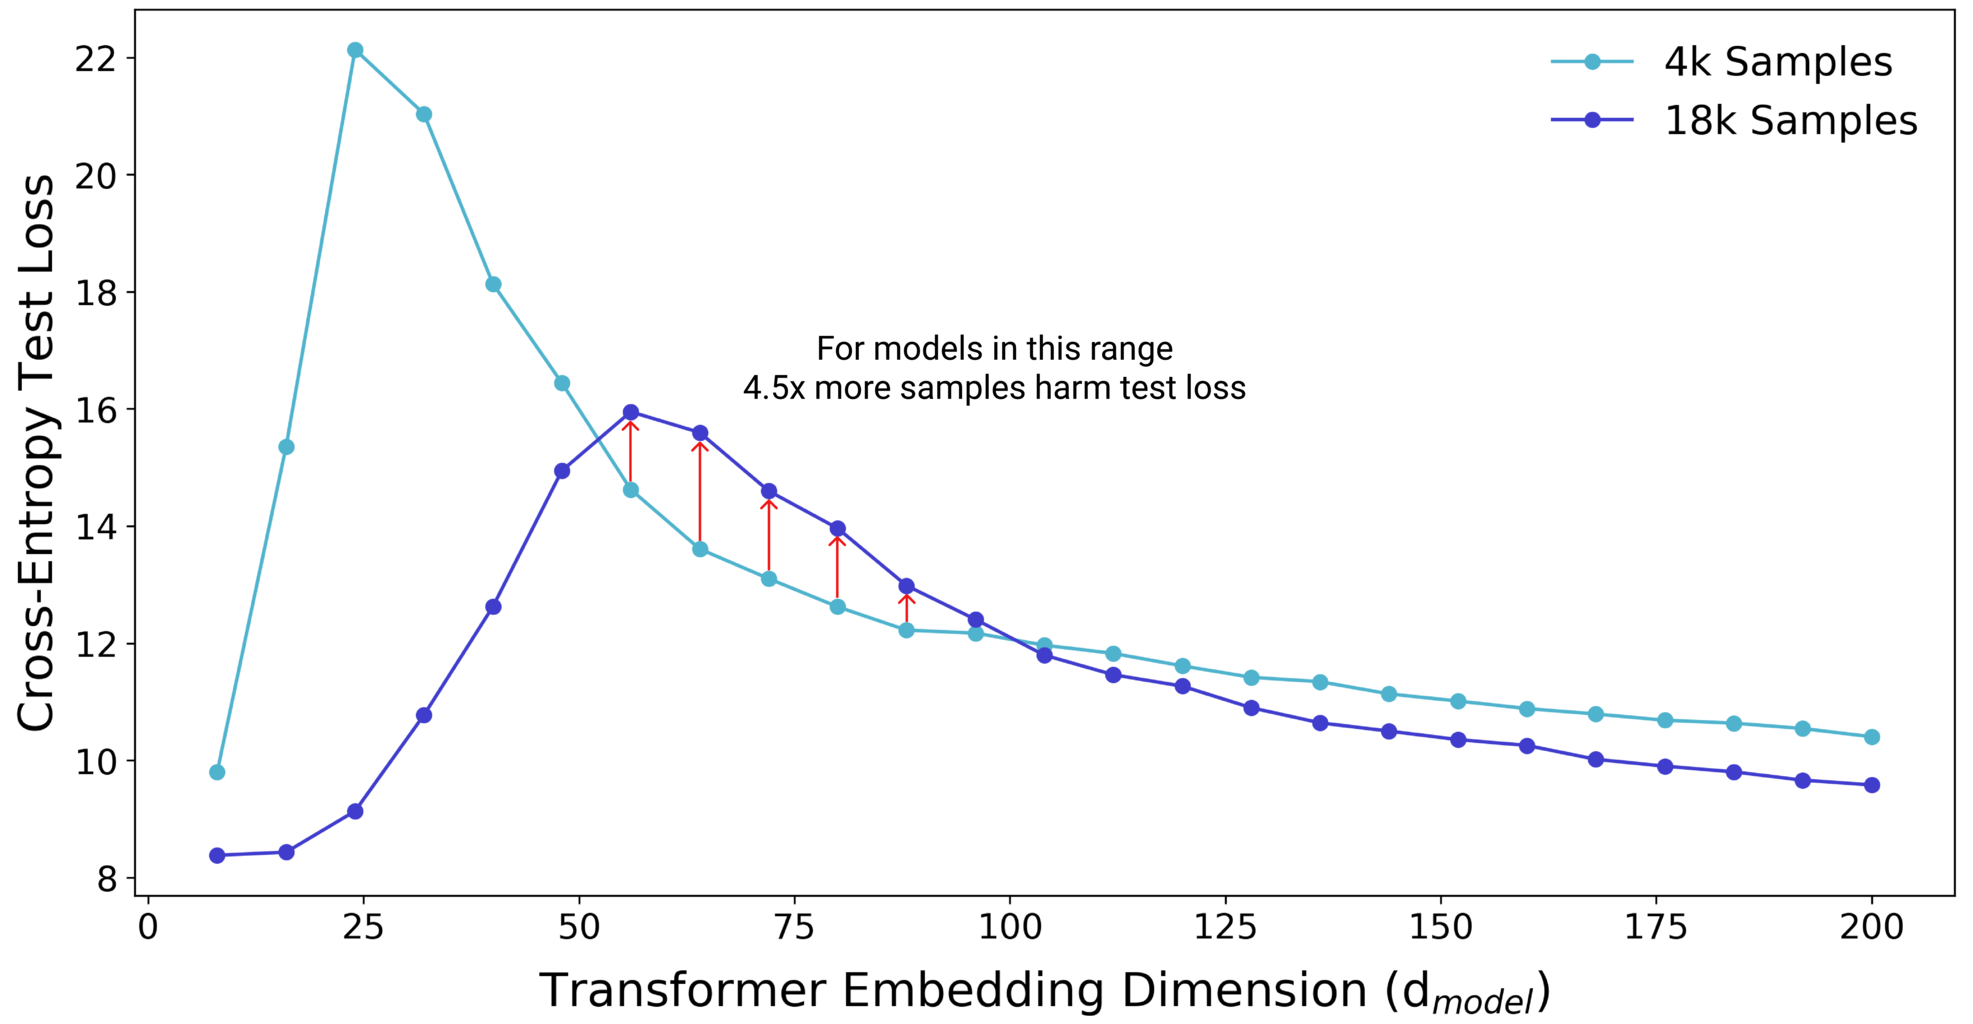
\includegraphics[width=0.95\linewidth,height=4.4cm,keepaspectratio]{assets/NLP-small-data-vary-MDD.png}\\[0.1ex]
{\scriptsize\color{uommuted}\textbf{Fig.~3, Nakkiran et al.} IWSLT'14 De-En, 6-layer Transformer, \(d_{\text{ff}}\!=\!4d_{\text{model}}\), 80k gradient steps, 10\% label smoothing. Highlighted bars indicate the \(d_{\text{model}}\) interval over which a 4.5\(\times\) increase in \(n\) \emph{raises} test loss.}
\justifying
\vspace{0.1ex}
\begin{itemize}\setlength\itemsep{0.2ex}
\item Fixing \((\T,\F)\) and increasing \(n\) leaves the interpolation threshold in EMC space unchanged but shifts \(n\) relative to it; widths near the small-sample threshold are thereby displaced into the critical regime.
\item The non-monotonicity is local: asymptotically, additional samples reduce excess risk.
\end{itemize}
\end{block}
\end{column}

% --------- RIGHT: MECHANISM ---------
\begin{column}{0.485\linewidth}
\begin{block}{6.~Mechanism and implication chain (rigorous for linear models; conjectural for deep nets)}
\eyebrow{Critically parameterised} \(\;\)The hypothesis class admits effectively a unique interpolant. Constraining it to fit noisy or mis-specified labels perturbs the on-distribution map; test risk consequently spikes.

\vspace{0.3ex}
\eyebrow{Over-parameterised} \(\;\)A continuum of interpolants exists. The optimiser's \kw{implicit bias} (e.g.\ SGD toward minimum-norm solutions) selects an interpolant that absorbs label noise while preserving smoothness on the data manifold.

\vspace{0.4ex}
\centering
\begin{tikzpicture}[every node/.style={font=\footnotesize},x=0.32\linewidth,y=0.75cm]
  \shade[left color=accentteal!20, right color=accentcoral!55] (0,0) rectangle (1,0.5);
  \shade[left color=accentcoral!55, right color=accentgreen!25] (1,0) rectangle (2.5,0.5);
  \draw[->,thick] (0,-0.05) -- (2.6,-0.05) node[right] {\color{uommuted}\footnotesize increasing \(\mathrm{EMC}\)};
  \node[anchor=south] at (0.5,0.5) {\bfseries unique interpolant};
  \node[anchor=south] at (1.0,0.6) {\bfseries\color{accentcoral}\(\approx n\)};
  \node[anchor=south] at (1.75,0.5) {\bfseries continuum of interpolants};
  \node[anchor=north] at (0.5,0) {classical U-curve};
  \node[anchor=north,color=accentcoral] at (1.0,-0.15) {peak};
  \node[anchor=north] at (1.75,0) {implicit bias selects};
\end{tikzpicture}

\justifying
\vspace{0.3ex}
\eyebrow{Where the mechanism is proven}
\(\;\)Mei \& Montanari (2022, Thm.~2) establish a test-risk peak at \(d{=}n\) for random-features regression under mis-specification; Belkin et al.\ (2019) prove an analogous peak for least-squares; Bartlett et al.\ (2020) prove benign overfitting under minimum-norm interpolation. The deep-network analogue remains conjectural.

\vspace{0.3ex}
\eyebrow{Implication chain}
\(\;\)Decreasing \(n\) at fixed \(\T\) increases \(\mathrm{EMC}/n\), shifting the regime further into over-parameterisation; an \kw{ensemble of \(K\) models trained on disjoint sub-samples} therefore lies past each member's peak, and averaging cancels member-specific interpolation noise (Nakkiran et al., Fig.~28).
\end{block}
\end{column}
\end{columns}

\vspace{-0.25cm}

% =====================================================================
% TWO-COLUMN ROW: What we don't claim | Practice + Open
% =====================================================================
\begin{columns}[T,onlytextwidth]

% --------- LEFT: WHAT WE DON'T CLAIM ---------
\begin{column}{0.485\linewidth}
\begin{block}{7.~Critical reflection: what we do \emph{not} claim}
\begin{itemize}\setlength\itemsep{0.2ex}
\item \kw{The bias-variance trade-off is not invalidated.} It remains correct within a fixed hypothesis class; it is \emph{incomplete} once \(\T\) is permitted to vary.
\item \kw{Capacity, training time, and sample size are not monotonic.} Within the critical interval each can locally \emph{increase} test risk.
\item \kw{Label noise is not the cause of the peak.} Noise amplifies it; the peak persists at \kw{0\% noise} (CIFAR-100, Fig.~4a; CNN, Fig.~7) under model mis-specification.
\item \kw{Parameter count does not equal capacity.} Parameters constitute one input to EMC; optimiser, epochs, augmentation, and label policy contribute jointly.
\end{itemize}
\end{block}
\end{column}

% --------- RIGHT: PRACTICE + OPEN ---------
\begin{column}{0.485\linewidth}
\begin{block}{8.~Practical implications and open questions}
\eyebrow{Implications for practice}
\begin{itemize}\setlength\itemsep{0.15ex}
\item \kw{Diagnostic.} Train and test curves decouple near the interpolation threshold; monitor both.
\item \kw{Per-model mitigation.} Weight decay, early stopping, or scaling well beyond the threshold.
\item \kw{Aggregate mitigation.} Ensemble \(K\) sub-sampled models, each over-parameterised relative to its own \(n\) (Fig.~28).
\item \kw{Augmentation.} Data augmentation shifts the peak rightward (Fig.~5) without changing the architecture.
\end{itemize}
\eyebrow{Open scientific questions}
\begin{itemize}\setlength\itemsep{0.15ex}
\item A principled choice of \(\varepsilon\) and closed-form critical-interval width.
\item A non-linear EMC theorem for over-parameterised networks.
\item Characterisation of SGD's implicit bias for realistic architectures and losses.
\end{itemize}
\end{block}
\end{column}
\end{columns}

\vspace{-0.15cm}
\bigtakeaway{Interpolation is a threshold to understand, not a final verdict.}
\vspace{-0.05cm}

% =====================================================================
% FOOTER: References + AI declaration (full width, two columns)
% =====================================================================
\begin{columns}[T,onlytextwidth]
\begin{column}{0.66\linewidth}
\eyebrow{Key references}\vspace{-0.7ex}
{\scriptsize
[1]~Nakkiran, Kaplun, Bansal, Yang, Barak, Sutskever. \emph{Deep Double Descent: Where Bigger Models and More Data Hurt.} arXiv:1912.02292 (2019). \;
[2]~Belkin, Hsu, Ma, Mandal. \emph{Reconciling modern ML practice and the classical bias-variance trade-off.} PNAS 116(32) (2019). \;
[3]~Zhang, Bengio, Hardt, Recht, Vinyals. \emph{Understanding deep learning requires rethinking generalization.} ICLR (2017). \;
[4]~Mei \& Montanari. \emph{The generalization error of random features regression.} Comm.\ Pure Appl.\ Math.\ (2022). \;
[5]~Bartlett, Long, Lugosi, Tsigler. \emph{Benign overfitting in linear regression.} PNAS 117(48) (2020). \;
[6]~Brown \& Mukherjee. \emph{COMP34312 Notes 2026, \S\,5}.
}
\end{column}
\begin{column}{0.32\linewidth}
\eyebrow{AI-use declaration}\vspace{-0.5ex}
{\scriptsize
Generative AI was used solely as a \LaTeX{} typesetting assistant for the poster source. All conceptual content, figure choices, mathematical claims, and source references were directed and verified by the authors. Figures 1\textendash 3 are reproduced from Nakkiran et al.\ (2019).
}
\end{column}
\end{columns}

\end{frame}
\end{document}
